\section{Исследование моделей}
\label{sec:Chapter4} \index{Chapter4}

В данной главе будет представлено описание и результаты исследования моделей: BlazePose, MoveNet.SinglePose, OpenPose и MMPose.


\subsection{Описание эксперимента}

Эксперимент включает рассмотрение только моделей распознавания ключевых точек на теле человека, так как это является основной частью решения задачи классификации движений и многие классификаторы движений строятся на выходных данных о позе.

Из представленных в \autoref{subsec:pose_estimation_models} моделей были выбраны 4 представителя по некоторым критериям:

\begin{itemize}
	\item Доступность модели для исследований\\
	Необходимо оценить длительность установки и возможности работы с различными операционными системами. Эксперимент проводился на платформе Google Colab, поэтому необходимо было рассмотреть возможность использования модели на в Colaboratory.
	\item Новизна модели\\
	Представленная выборка была создана в основном в 2010-х, но модель DeepPose является самой старой. Новые разработки опирались на результаты, полученные в ней, и таким образом получали более хорошие результаты.
	\item Наличие документации\\
	Все модели производят классификацию по двум осям изображения: высота и ширина, а также по параметру видимость ключевой точки. Некоторые модели выдают данные нормированные на размер изображения (число из отрезка [0,1]), а некоторые точное значение в пикселях. Поэтому для работы необходимо было понимать как работает API модели, какие у нее входные - выходные данные.
	\item Тренировка модели на датасете COCO\\
	Все используемые претренированные модели были обучены на наборе данных COCO \cite{COCO_topology} в совместительстве с каким-либо другим датасетом. В некоторых  примерах не было возможности использовать претренированную модель и из-за этого они были отсеяны.
\end{itemize}

В итоге было выбрано 4 модели наиболее подходящие под критерии:
\begin{enumerate}
	\item BlazePose
	\item MoveNet.SinglePose
	\item OpenPose
	\item MMpose
\end{enumerate}

Для проведения качественного анализа и выявления лучшей модели необходимо их сравнить. Поэтому рассмотрим метрики, которые подходят для задач в 2-х мерном пространстве:

\begin{itemize}
	\item Percentage of Detection Joints\\
	PDJ оценивает точность распознавания ключевой точки в зависимости от диагональных размеров человека. При рассмотрении задачи распознавания человека на выходе имеются координаты точек, которые характеризуют прямоугольник, внутри которого вписан человек. Диагональ этого прямоугольника используется при высчитывании метрики PDJ (см. \autoref{fig:PDJ}). Формулу можно представить в следующем виде:
	\begin{equation}
		PDJ = \frac{\sum_{i=1}^{n} bool(d_i < threshold * diag)}{n},
	\end{equation}
	
	где\\
	$d_i$ - расстояние между предсказанной и правильной точкой,\\
	$threshold$ - порог, задаваемый исследователем,\\
	$diag$ - размер диагонали прямоугольника, внутри которого находится человек,\\
	$bool()$ - логическое условие, возвращает 1, если оно верно и 0 в ином случае,\\
	$n$ - размер выборки.
	
	С помощью значения порога можно варьировать допустимую погрешность расстояния между истинной и предсказанной точками.
	\begin{figure}[h]
		\centering
		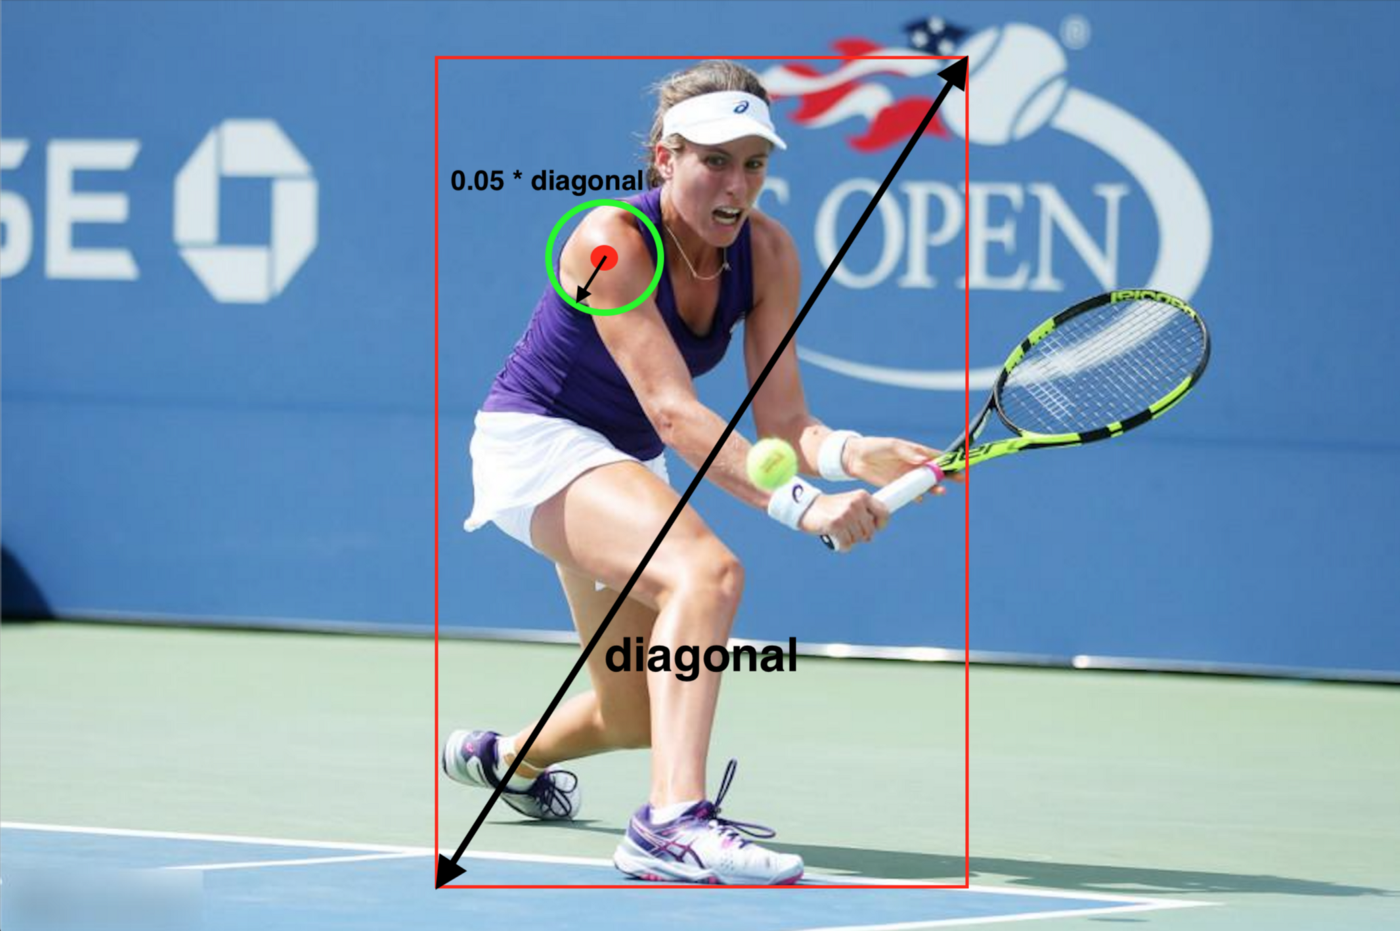
\includegraphics[width=\textwidth * 4 / 5]{./images/PDJ}
		\caption{Визуальное представление метрики PDJ.\\ Зеленый круг ограничивает область допустимого расположения распознанной ключевой точки.}
		\label{fig:PDJ}
	\end{figure}

	\item Percentage of Correct Key-points\\
	PCK очень похожа на предыдущую метрику, только погрешность рассматривается относительно высоты человека. Формулу можно представить в следующем виде:
	\begin{equation}
		PCK = \frac{\sum_{i=1}^{n} bool(d_i < threshold * body_height)}{n},
	\end{equation}
	
	где\\
	$d_i$ - расстояние между предсказанной и правильной точкой,\\
	$threshold$ - порог, задаваемый исследователем,\\
	$body_height$ - высота прямоугольника, внутри которого находится человек,\\
	$bool()$ - логическое условие, возвращает 1, если оно верно и 0 в ином случае,\\
	$n$ - размер выборки.
	
	\item Object Key-point Similarity\\
	OKS является основной при оценке задачи Keypoint Detection COCO \cite{COCO_topology}. Она использует третью координату выходного предсказания и расстояние между реальной и предсказанной точками. Формулу можно представить в следующем виде:
	\begin{equation}
		OKS = \frac{\sum_{i} exp\left( - d_i^2 / 2s^2k_i^2\right)\delta\left(v_i > 0\right)}{\sum_{i} \delta\left(v_i > 0\right)},
	\end{equation}
	где\\
	$d_i$ - расстояние между предсказанной и правильной точкой,\\
	$s$ - площадь объекта,\\
	$k_i$ - константа ключевой точки, контролирующаю спад,\\
	$v_i$ - видимость.
	
	При оценке задачи детекции ключевых точек COCO вводится метрика Average Precision (AP) через OKS. Изменяя границу допустимого значения OKS можно получать различные значения precision и AP.
\end{itemize}

В метриках PCK и PDJ необходимо знать размеры прямоугольника, ограничивающего человека. Для этого необходимо использовать модель распознавания объектов, которая будет давать нам эти данные. При работе с метрикой PCK можно обойтись без такой модели, потому что во всех топологиях есть точки, которые обозначают верхнюю и нижнюю границы человека. Отсюда погрешность вычисления через модель и вычисления разности ординат верхней и нижней точек будет мала. Что требует меньше затрат для оценки.

\subsection{Поиск данных}

Первым делом необходимо было проверить модели на неразмеченных данных. Для этого были выбраны фотографии высокого разрешения, где человек изображен во весь рост (см. \autoref{fig:test_photos}).

\begin{figure}[h]
\begin{subfigure}[b]{.5\textwidth}
	\centering
	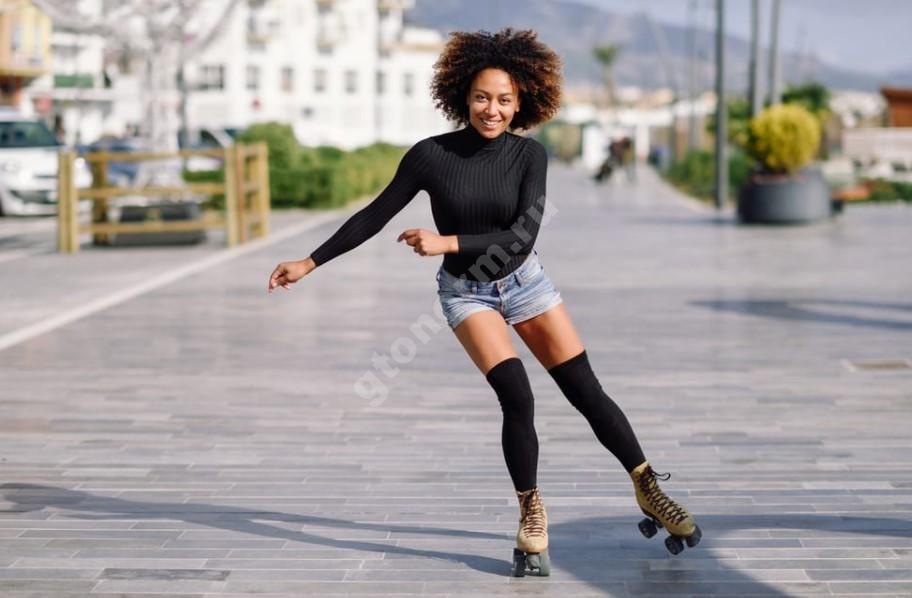
\includegraphics[width=\textwidth]{./images/Test/ролики2}
	\caption{ }
\end{subfigure}
\begin{subfigure}[b]{.5\textwidth}
	\centering
  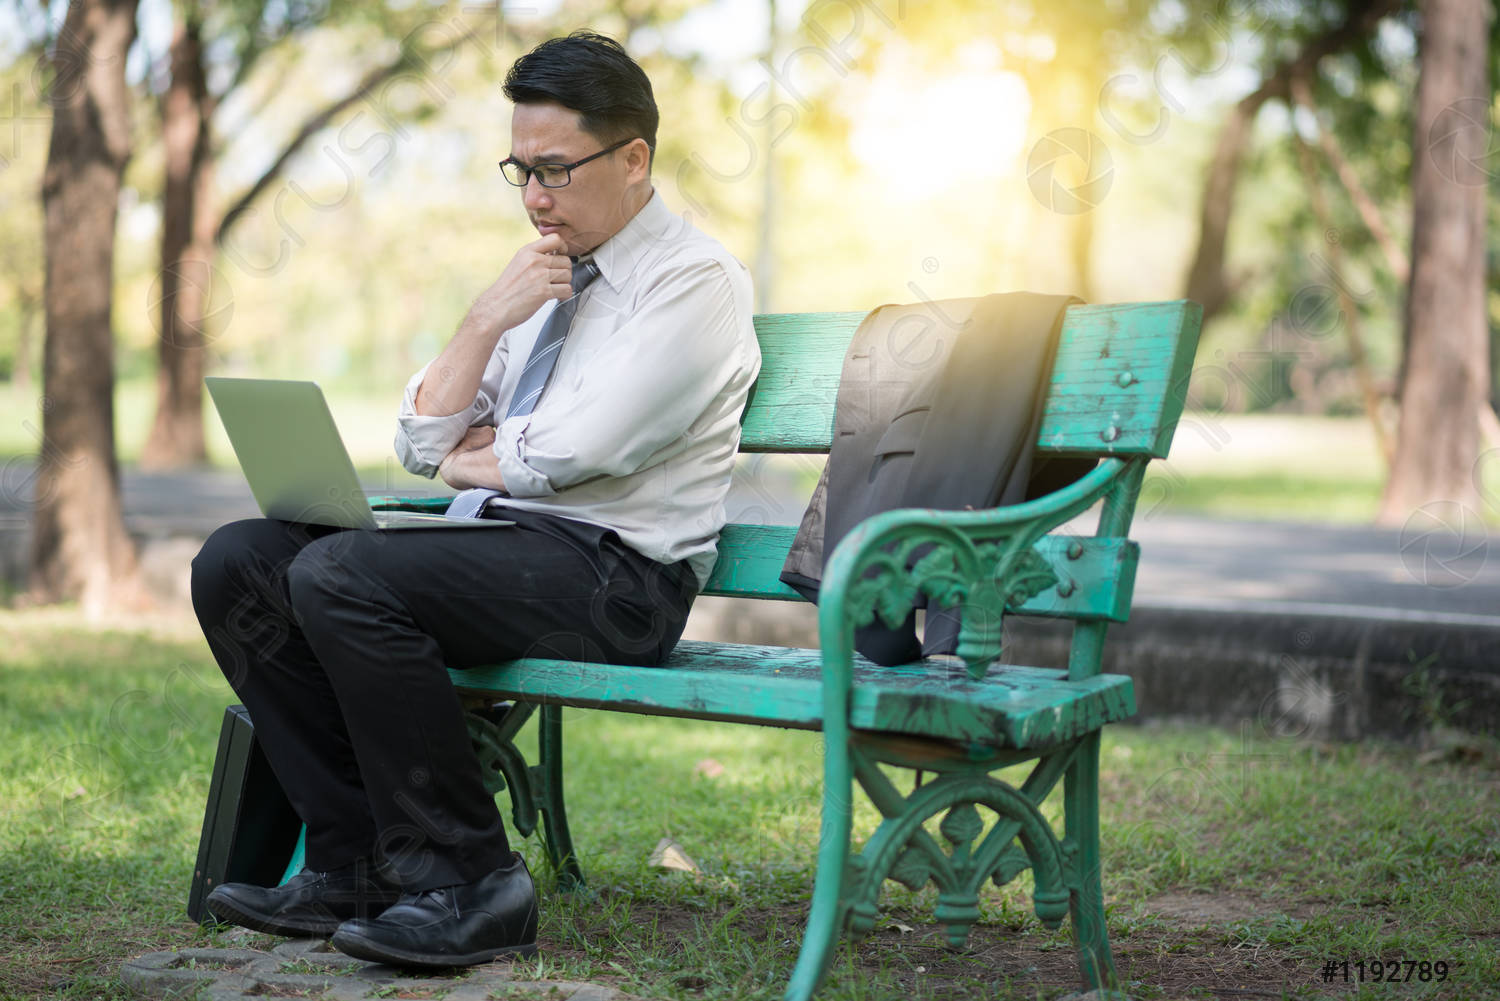
\includegraphics[width=\textwidth]{./images/Test/скамека3}
  \caption{ }
\end{subfigure}
\begin{subfigure}[b]{.5\textwidth}
	\centering
  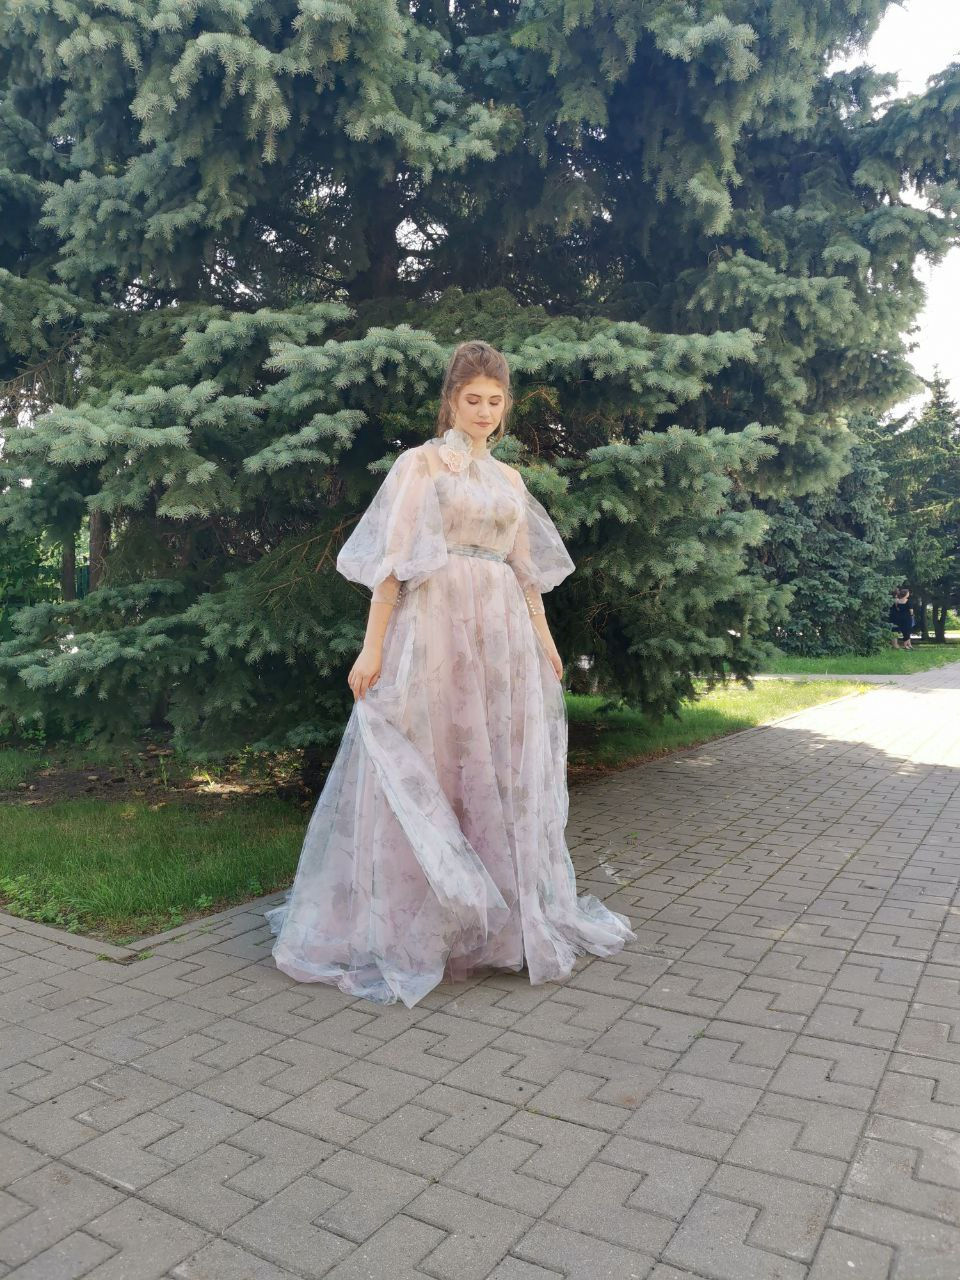
\includegraphics[height=\textwidth]{./images/Test/dress}
  \caption{ }
\end{subfigure}
\begin{subfigure}[b]{.5\textwidth}
	\centering
  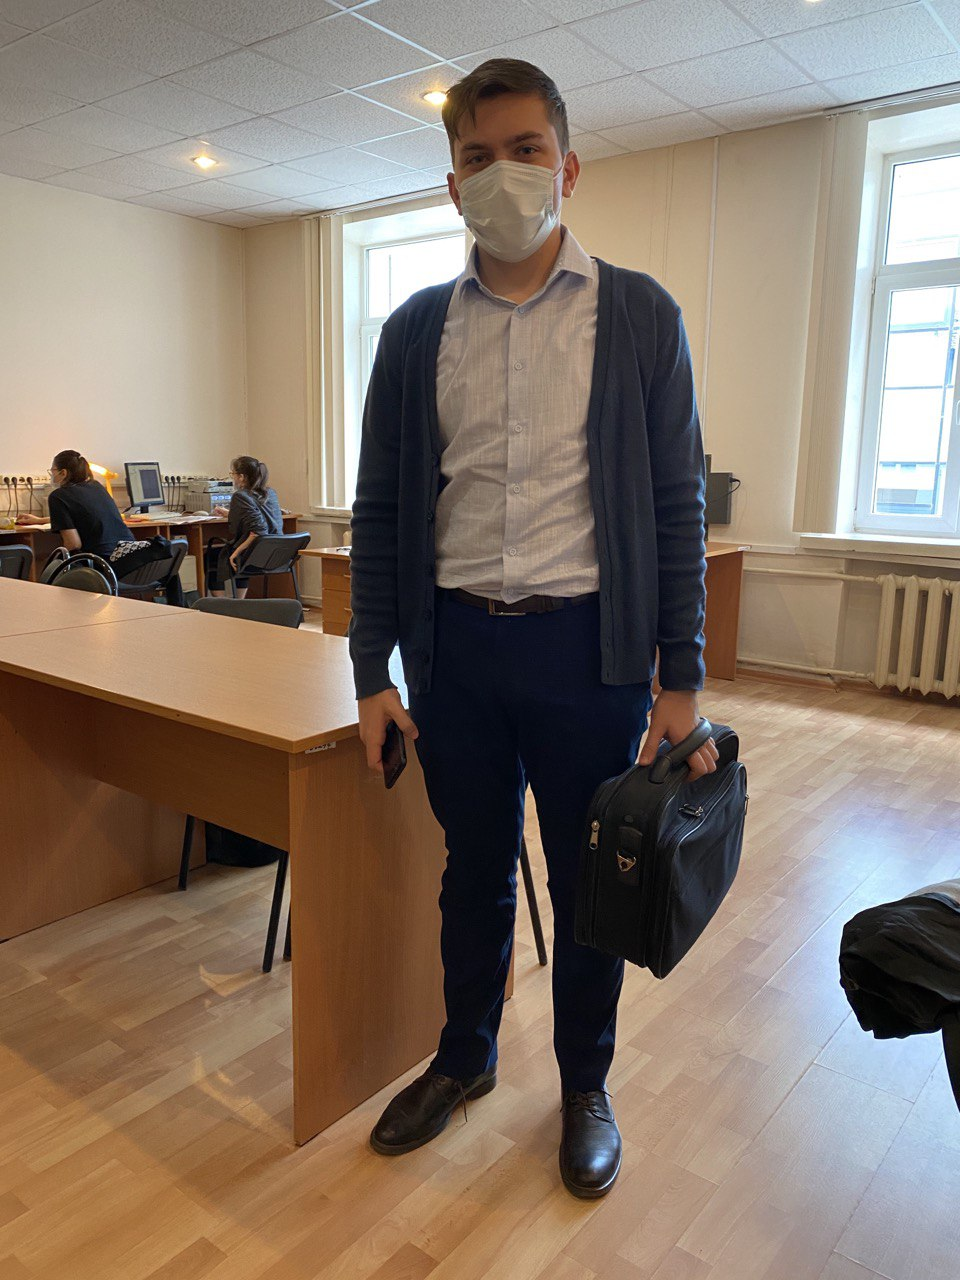
\includegraphics[height=\textwidth]{./images/Test/static}
  \caption{ }
\end{subfigure}
  \caption{Изображения для визуальной оценки моделей.}
  \label{fig:test_photos}
\end{figure}

Для качественной оценки работы моделей с помощью метрик необходимо было найти размеченные данные. Приведу описание датасетов, которые были мной рассмотрены:

\begin{itemize}
	\item COCO Dataset и MPII\\
	Данные наборы являются основными при работе с компьютерным зрением и большинство исследователей используют их как тренировочные для своих моделей. Поэтому использовать их в качестве тестовых не целесообразно. \cite{COCO_dataset, MPII_dataset}
	\item HUMAN 3.6M\\
	Данные собирались специально для задачи классификации движений человека в студии. С помощью датчиков фиксировались положения всех суставов и ключевых точек. Это идеальный датасет, но доступ к нему ограничен и создатель не выходит на связь. \cite{h36m_pami}
	\hfill \break
	\item LSP\\
	Данные собраны со спортивных соревнований и пред обработаны до обозначения одного человека на изображении размером не менее 150 пикселей в высоту. Единственная проблема - не описаны точки на лице, поэтому оценивать можно только распознавание 12 суставов или, другими словами, точек на теле человека. \cite{LSP}
	\item LSP Extended\\
	Является расширенной версией предыдущего набора данных. По объёму превосходит его в пять раз. Остальные характеристики не поменялись. \cite{LSPE}
	\item Halpe\\
	Датасет для распознавания точек на всем теле человека. К каждой фотографии идет аннотация из 136 точек, краев ограничивающего прямоугольника и категории детектируемого объекта (во всех фотографиях стоит категория человек).
	
	Набор состоит из двух частей: HICO-DET и COCO. Все они аннотированны описанные выше способом. Для наших моделей необходимо будет отобрать только 17 точек, совпадающих с топологией СОСО. \cite{Halpe_dataset}
\end{itemize}

Выше были представлены наборы данных для задачи распознавания точек на теле человека. Но основной темой является классификация движений человека, поэтому необходимы фотографии с меткой класса для позы, представленной на данных. Некоторые из уже представленных (COCO, MPII) тоже могут использоваться для классификации позы, но по тем же причинам, что и описаны выше, они не будут рассмотрены в эксперименте. Приведу описание датасетов для классификации движения человека по позе на изображении:


\begin{itemize}
	\item Stanford-40\\
	Набор данных состоит примерно из 10 тыс. изображений, на каждом из которых человек делает одно из 40 действий. На один класс приходится от 180 до 300 фотографий. \cite{stanford40}
	\item Yoga-82\\
	Сложность распознавания поз йоги в том, что многие из них не могут быть точно аннотированы. Для решения этой проблемы и был собран этот набор данных вмещающий примерно 28 тыс. изображений. 82 различные позы разделены по 6 подклассам. При желании можно использовать метки и классов, и подклассов для классификации. \cite{verma2020yoga}
\end{itemize}

Итого были выбраны наборы данных LSP, LSPE и Halpe. \begin{figure}[h]
\begin{subfigure}[b]{.2\textwidth}
	\centering
	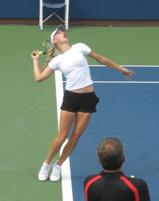
\includegraphics[height=\textwidth]{./images/LSP1}
\end{subfigure}
\begin{subfigure}[b]{.1\textwidth}
	\centering
  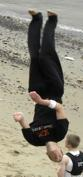
\includegraphics[height=2\textwidth]{./images/LSP2}
\end{subfigure}
\begin{subfigure}[b]{.2\textwidth}
	\centering
  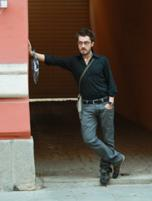
\includegraphics[height=\textwidth]{./images/LSP3}
\end{subfigure}
\begin{subfigure}[b]{.15\textwidth}
	\centering
  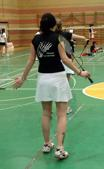
\includegraphics[height=4\textwidth / 3]{./images/LSP4}
\end{subfigure}
\begin{subfigure}[b]{.15\textwidth}
	\centering
  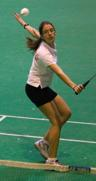
\includegraphics[height=4\textwidth / 3]{./images/LSP5}
\end{subfigure}
\begin{subfigure}[b]{.15\textwidth}
	\centering
  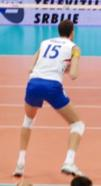
\includegraphics[height=4\textwidth / 3]{./images/LSP6}
\end{subfigure}
  \caption{Примеры изображений из датасета LSP.}
  \label{fig:dataset_photos}
\end{figure}

\subsection{Результаты эксперимента}

Для каждой модели была рассмотрена локализация ключевых точек на фотографиях высокого качества (см. \autoref{fig:test_photos}), а также набор данных низкого качества с обработанными изображениями.

Метрики были рассчитаны с порогами 0.05, 0.2, 0.5. В дополнение к этому был проведен временной анализ классификации одного изображения в среднем по целому датасету.

Перейдем к результатам по каждой модели.
\hfill \break

\textbf{
	\begin{large}
		BlazePose
	\end{large}
}

Результаты работы модели можно посмотреть на \autoref{fig:MP_result}. Как можно заметить, некоторые точки не распознаются и не отображаются на итоговом результате. А также есть небольшая погрешность при распознавании глаз. Но модель хорошо сработала на человека в маске.

Исходя из значений метрик (см. в \autoref{tab:MP_table}) можно сделать вывод, что модель имеет высокую погрешность при среднем времени обработки одной фотографии 0.076 секунды.

\begin{table}[h]
	\centering
	\begin{tabular}{|p{1.5cm}||p{2.2cm}|p{2cm}|p{2cm}|p{2.2cm}|p{2cm}|p{2cm}|}
		\hline
		Metric&PCK@0.05&PCK@0.2&PCK@0.5&PDJ@0.05&PDJ@0.2&PDJ@0.5\\\hline
		\hline
		LSP & 0.728 & 0.931 & 0.978 & 0.773 & 0.944 & 0.988\\
		LSPE & 0.454 & 0.743 & 0.825 & 0.557 & 0.783 & 0.851\\
		Halpe & 0.365 & 0.519 & 0.595 & 0.417 & 0.554 & 0.638\\
		\hline
	\end{tabular}
	\begin{tabular}{|p{1.5cm}||p{2cm}|p{2cm}|p{2cm}|}
		\hline
		Metric&AP@0.5&AP@0.75&AP\\\hline\hline
		LSP & 0.184 & 0.093 & 0.1\\
		LSPЕ & 0.675 & 0.457 & 0.443\\
		Halpe & 0.33 & 0.158 & 0.173\\
		\hline
	\end{tabular}
	\caption{Результаты вычисления метрик для BlazePose.}
	\label{tab:MP_table}
\end{table}
\hspace{1cm}

\textbf{
	\begin{large}
		MoveNet.SinglePose
	\end{large}
}

Результаты работы модели можно посмотреть на \autoref{fig:MN_result}. Заметны огрехи в распознавании локтей и ладоней. Как и в прошлой модели есть неточности при распознавании частей лица.

Исходя из значений метрик (см. в \autoref{tab:MN_table}) можно сделать вывод, что модель показала себя плохо при оценивании с порогом 0.05, но лучший результат среди всех для порогах 0.2 и 0.5. Среднее время обработки одной фотографии составило 0.028 секунды, что также является наилучшим показателем.

\begin{table}[h]
	\centering
	\begin{tabular}{|p{1.5cm}||p{2.2cm}|p{2cm}|p{2cm}|p{2.2cm}|p{2cm}|p{2cm}|}
		\hline
		Metric&PCK@0.05&PCK@0.2&PCK@0.5&PDJ@0.05&PDJ@0.2&PDJ@0.5\\\hline
		\hline
		LSP & 0.356 & 0.928 & 0.983 & 0.43 & 0.95 & 0.993\\
		LSPE & 0.144 & 0.539 & 0.745 & 0.227 & 0.635 & 0.806\\
		Halpe & 0.04 & 0.052 & 0.223 & 0.006 & 0.078 & 0.32\\
		\hline
	\end{tabular}
	\begin{tabular}{|p{1.5cm}||p{2cm}|p{2cm}|p{2cm}|}
		\hline
		Metric&AP@0.5&AP@0.75&AP\\\hline\hline
		LSP & 0.168 & 0.064 & 0.08\\
		LSPЕ & 0.312 & 0.059 & 0.111\\
		\hline
	\end{tabular}
	\caption{Результаты вычисления метрик для MoveNet.SinglePose.}
	\label{tab:MN_table}
\end{table}


\textbf{
	\begin{large}
		OpenPose
	\end{large}
}

Результаты работы модели можно посмотреть на \autoref{fig:OP_result}.

Значения метрик см. в \autoref{tab:OP_table}.

Среднее время обработки одной фотографии составило 0.072 секунды.

Визуально лучший результат обработки изображений, хотя по метрикам немного уступает следующей модели. Но полностью обыгрывает ее во времени обработки.

\begin{table}[h]
	\centering
	\begin{tabular}{|p{1.5cm}||p{2.2cm}|p{2cm}|p{2cm}|p{2.2cm}|p{2cm}|p{2cm}|}
		\hline
		Metric&PCK@0.05&PCK@0.2&PCK@0.5&PDJ@0.05&PDJ@0.2&PDJ@0.5\\\hline
		\hline
		LSP & 0.708 & 0.837 & 0.882 & 0.746 & 0.845 & 0.899\\
		LSPE & 0.362 & 0.524 & 0.633 & 0.42 & 0.569 & 0.69\\
		Halpe & 0.575 & 0.638 & 0.686 & 0.613 & 0.658 & 0.72\\
		\hline
	\end{tabular}
	\begin{tabular}{|p{1.5cm}||p{2cm}|p{2cm}|p{2cm}|}
		\hline
		Metric&AP@0.5&AP@0.75&AP\\\hline\hline
		LSP & 0.166 & 0.085 & 0.092\\
		LSPЕ & 0.538 & 0.362 & 0.362\\
		Halpe & 0.562 & 0.398 & 0.384\\
		\hline
	\end{tabular}
	\caption{Результаты вычисления метрик для OpenPose.}
	\label{tab:OP_table}
\end{table}

\textbf{
	\begin{large}
		MMPose
	\end{large}
}

Результаты работы модели можно посмотреть на \autoref{fig:MMP_result}.

Значения метрик см. в \autoref{tab:MMP_table}.

Среднее время обработки одной фотографии составило 0.675 секунды.

Для своей работы требует детекции человека, из-за чего показывает лучший результат в точности, но худший результат по времени обработки одного изображения.

\begin{table}[h]
	\centering
	\begin{tabular}{|p{1.5cm}||p{2.2cm}|p{2cm}|p{2cm}|p{2.2cm}|p{2cm}|p{2cm}|}
		\hline
		Metric&PCK@0.05&PCK@0.2&PCK@0.5&PDJ@0.05&PDJ@0.2&PDJ@0.5\\\hline
		\hline
		LSP & 0.728 & 0.85 & 0.914 & 0.76 & 0.858 & 0.933\\
		LSPE & 0.403 & 0.56 & 0.651 & 0.463 & 0.587 & 0.72\\
		Halpe & 0.418 & 0.478 & 0.532 & 0.451 & 0.498 & 0.574\\
		\hline
	\end{tabular}
	\begin{tabular}{|p{1.5cm}||p{2cm}|p{2cm}|p{2cm}|}
		\hline
		Metric&AP@0.5&AP@0.75&AP\\\hline\hline
		LSP & 0.225 & 0.223 & 0.123\\
		LSPЕ & 0.598 & 0.462 & 0.443\\
		Halpe & 0.65 & 0.534 & 0.502\\
		\hline
	\end{tabular}
	\caption{Результаты вычисления метрик для MMPose.}
	\label{tab:MMP_table}
\end{table}
\hfill \break

\textbf{
	\begin{large}
		Графики результатов
	\end{large}
}

На \autoref{fig:results_pck} и \autoref{fig:results_pdj} представлены средние для трех датасетов (LSP, LSPE и Halpe) метрик PCK и PDJ соответственно. Модель BlazePose является явным лидером. OpenPose и MMPose хоть и имеют такие же значения метрик при маленьком пороге, но медленнее увеличивают качество распознавания с ростом допустимой погрешности. MoveNet при всей своей скорости работы похожа на BlazePose только трендом изменения метрики, но не результатами.

\begin{figure}[h]
	\centering
	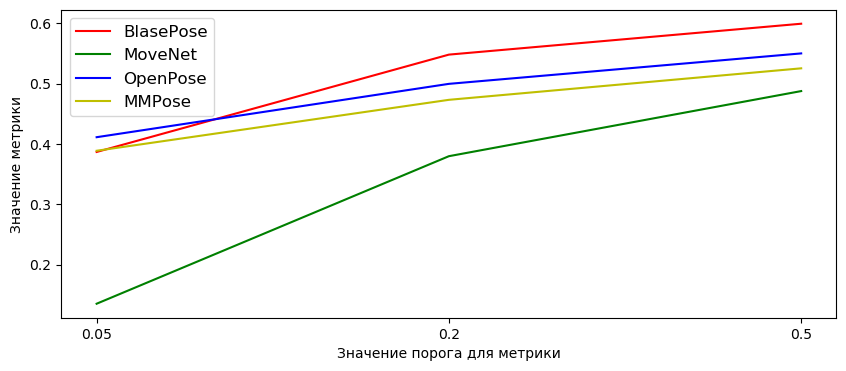
\includegraphics[width=0.97\textwidth]{./images/results/PCK}
	\caption{Средние значения метрики PCK.}
	\label{fig:results_pck}
\end{figure}

Результаты растут с увеличением порога, так как увеличивается и допустимая погрешность локализации. Следовательно и количество верных точек тоже становится больше. При пороге 0.5 качество распознавания у всех моделей примерно выравнивается.

\begin{figure}[h]
	\centering
   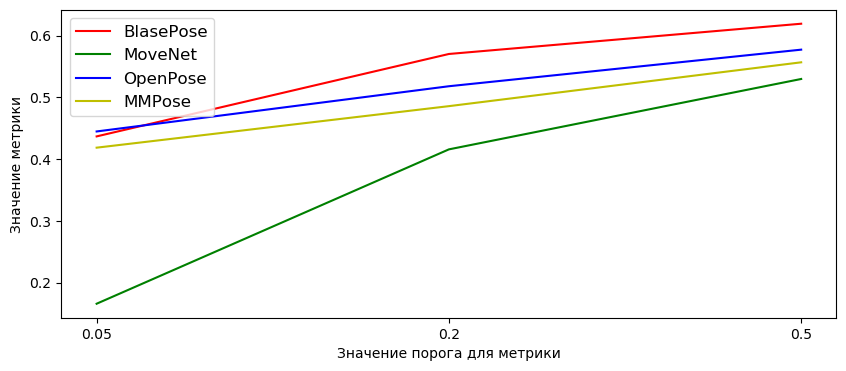
\includegraphics[width=0.97\textwidth]{./images/results/PDJ}
   \caption{Средние значения метрики PDJ.}
   \label{fig:results_pdj}
\end{figure}

На \autoref{fig:results_ap} представлены значения метрики AP также по всем трем наборам данных. Модель MoveNet так и показывает довольно плохой результат работы во многом за счет плохого результата на изображениях из Halpe. Модель MMPose показывает много лучший результат работы, в отличие от двух других, которые так и держатся рядом на графиках.

\begin{figure}[h]
	\centering
   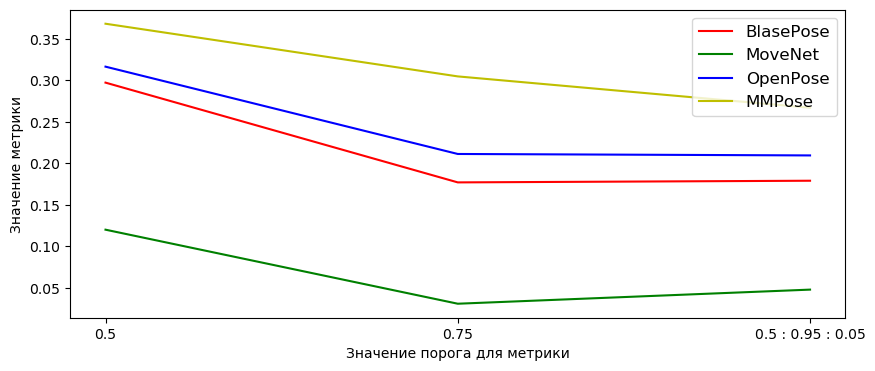
\includegraphics[width=0.97\textwidth]{./images/results/AP}
   \caption{Средние значения метрики AP.}
   \label{fig:results_ap}
\end{figure}

Результаты данной метрики убывают, так как с увеличением порога метрики растет минимально допустимое значение OKS, которое необходимо для определения верного распознавания.




\newpage
